\section{Durchführung}
\label{sec:Durchführung}
Der für den Versuch verwendete Aufbau ist in \autoref{fig:aufbau} dargestellt.
Die Ladungsimpulse im Zählrohr fließen über einen Widerstand $R$ ab und erzeugten
dort einen Spannungsimpuls. Dieser Spannungsimupls wird mithilfe eines
Kondensators entkoppelt und über einen Verstärker vergrößert.
Mit einem Zählgerät wird dann die Anzahl an Spannungsimpulsen aufgezeichnet, außerdem
kann deren Verlauf über ein Oszilloskop beobachtet werden.

\begin{figure}[H]
    \centering
    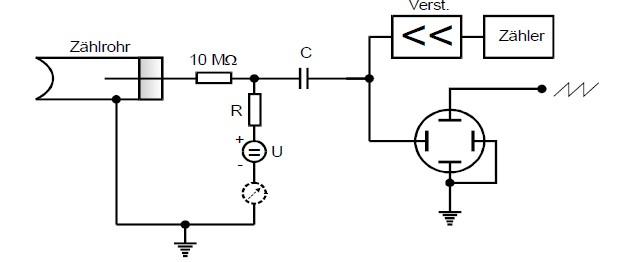
\includegraphics[height=5cm]{content/pics/aufbau.jpg}
    \caption{Skizze des Versuchsaufbaus. \cite{v703}.}
    \label{fig:aufbau}
\end{figure}

\subsection{Aufnahme der Zählrohrcharakteristik}
Vor dem Geiger-Müller-Zählrohr wird ein $\beta$-Strahler platziert.
Die Zählrohrspannung wird ausgehend von $\qty{300}{\volt}$ in $\qty{10}{\volt}$ Schritten erhöht,
bis der Maximalwert von $\qty{700}{\volt}$ erreicht ist.
Für jede Spannung wird die Impulsrate in einem Messzeitintervall von $\symup{\Delta}t=\qty{120}{\second}$
aufgenommen, sodass anschließend der Zusammenhang zwischen Zählrohrspannung und Impulsrate
gemäß \autoref{fig:gmz charakteristik} untersucht werden kann.
Außerdem wird zu jeder Spannung der Strom im Zählrohr notiert, der mithilfe eines dort angeschlossenen
Strommessgerätes abgelesen werden kann. Damit lässt sich die vom Zählrohr pro eindringendes Teilchen
freigesetzte Ladungsmenge bestimmen.

\subsection{Messung von Nachentladung und Totzeit}
Die Nachentladung sowie die Totzeit kann direkt aus einem Oszilloskopbild abgelesen werden.
Dafür wird mit dem selben $\beta$-Strahler bei einer Spannung von $\qty{500}{\volt}$
ein Oszilloskopbild erstellt. Es wird ein digitales Oszilloskop verwendet, dass an das
Strommessgerät für den Zählrohrstrom angeschlossen ist.

Die Totzeit wird außerdem über die \textit{Zwei-Quellen-Methode} bestimmt, sodass dieser Wert mit dem
zuvor abgelesenen Wert verglichen werden kann. Dafür werden ein starker und schwacher $\beta$-Strahler
verwendet, die zunächst einzelnd und dannach gemeinsam bei der Zählrohrspannung von $\qty{500}{\volt}$
gemessen werden.